\documentclass[12pt,a4paper]{article}
\usepackage{amsmath, amssymb}
\usepackage{graphicx}
\usepackage{fancyhdr}
\begin{document}
\pagestyle{fancy}
\fancyhf{}
\fancyhead[L]{
\includegraphics[height=1cm]{IIITB-COMET-Logo.png}}
\fancyhead[R]{Name:P.Muskan\\
ID:cometfwc035}
\begin{center}
\textbf{GATE CS-2010}
\end{center}

\section*{Q.31}
What is the Boolean expression for the output $f$ of the combinational logic circuit of NOR gates given below? 

\begin{center}
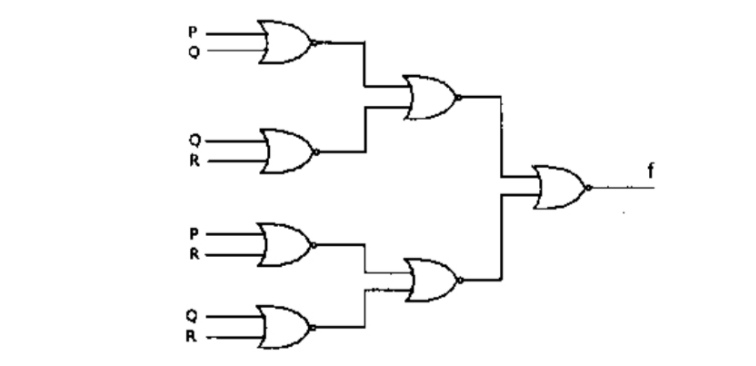
\includegraphics[width=0.6\textwidth]{31.jpg}
\end{center}

\noindent
\textbf{Options:}
\begin{enumerate}
\item[(A)] $\overline{Q + R}$
\item[(B)] $\overline{P + Q}$
\item[(C)] $\overline{P + R}$
\item[(D)] $\overline{P + Q + R}$
\end{enumerate}

\subsection*{Solution:}
Let each NOR gate output be analyzed step-by-step:

\begin{align*}
X_1 &= \overline{P + Q} \\
X_2 &= \overline{Q + R} \\
X_3 &= \overline{P + R} \\
X_4 &= \overline{Q + R} \\
Y_1 &= \overline{X_1 + X_2} 
    = \overline{\overline{P + Q} + \overline{Q + R}} \\
Y_2 &= \overline{X_3 + X_4} 
    = \overline{\overline{P + R} + \overline{Q + R}} \\
f &= \overline{Y_1 + Y_2}
\end{align*}

Using De Morgan's laws and simplification:

\[
Y_1 = \overline{\overline{P+Q} + \overline{Q+R}} 
     = (P+Q)(Q+R)
\]
\[
Y_2 = \overline{\overline{P+R} + \overline{Q+R}} 
     = (P+R)(Q+R)
\]
\[
f = \overline{(P+Q)(Q+R) + (P+R)(Q+R)}
\]

Factor $(Q+R)$:
\[
f = \overline{(Q+R)[(P+Q) + (P+R)]}
\]
\[
(P+Q) + (P+R) = P + Q + R
\]
So:
\[
f = \overline{(Q+R)(P+Q+R)}
\]
Since $(Q+R)(P+Q+R) = Q+R$ (absorption law):
\[
f = \overline{Q+R}
\]

\noindent
\textbf{Answer:} Option (A) $\quad \boxed{\overline{Q+R}}$
\end{document}

